% !TEX program = lualatex
\documentclass[aspectratio=169,professionalfonts]{beamer}
%------------------------- Preamble (beamer) -------------------------%
%   Require LuaLaTeX + --shell-escape (for minted)                    %
%--------------------------------------------------------------------%
\usepackage[spanish]{babel}

% ---------- Fonts (modern look) ----------
\usepackage{fontspec}
\defaultfontfeatures{Ligatures=TeX, Scale=MatchLowercase}
\setmainfont{Inter}       % Sans‑serif body (install ttf–Inter)
\setsansfont{Inter}
\setmonofont{Fira Code}   % Nice mono for code

% ---------- Theme ----------
\usetheme[
  titleformat=smallcaps,
  numbering=fraction,
  progressbar=frametitle   % thin progress line under the title
]{metropolis}              % modern beamer theme
\metroset{block=fill}      % coloured blocks

% ---------- Colours ----------
\definecolor{clblue}{HTML}{005F9E}
\definecolor{clorange}{HTML}{FF9130}
\definecolor{clgrey}{HTML}{F4F4F4}

% ---------- minted ----------
\usepackage{minted}
\setminted{
  fontsize=\footnotesize,
  autogobble,
  breaklines,
  tabsize=2,
  style=monokai,
  linenos
}

% ---------- Custom boxes (tcolorbox) ----------
\usepackage{tcolorbox}
\tcbuselibrary{skins, breakable}
% Warning box
\newtcolorbox{warnbox}{
  colback=clorange!10,
  colframe=clorange!80!black,
  breakable,
  title={\faWarning\quad Advertencia},
  fonttitle=\bfseries,
  left=2mm, right=2mm, top=1mm, bottom=1mm
}
% Information box
\newtcolorbox{infobox}{
  colback=clblue!5,
  colframe=clblue!60!black,
  breakable,
  title={\faInfoCircle\quad Nota},
  fonttitle=\bfseries,
  left=2mm, right=2mm, top=1mm, bottom=1mm
}

% ---------- Icons ----------
\usepackage{fontawesome5}

% ---------- Misc tweaks ----------
\graphicspath{{figures/}}
\setlength{\parskip}{0.5em}
\addto\extrasspanish{\renewcommand{\contentsname}{Índice}}
%--------------------------------------------------------------------%



\title[ClústerLab • Día 1]{Linux básico y primeros comandos}
\subtitle{Hands--on en Raspberry Pi 5}
\author{Equipo docente ClústerLab}
\date{4 de agosto de 2025}

\begin{document}

%---------------- title ----------------------------%
\begin{frame}[plain]
  \titlepage
\end{frame}

%---------------- SSH ------------------------------%
\begin{frame}[fragile]{Conectar a la Raspberry Pi}
  \begin{block}{Con pantalla y teclado}
    Usuario: \texttt{pi} \hfill Contraseña: \texttt{raspberry}
  \end{block}
  \begin{infobox}
    Para seguridad, cambia la contraseña en el primer login ↘︎
  \end{infobox}
  \begin{minted}{bash}
$ ssh pi@192.168.1.50        # IP de tu Pi
$ passwd #  cambiar contraseña (not necessary)
  \end{minted}
  \small Si usas Windows, conéctate desde Ubuntu WSL 2 o usa PuTTY.
\end{frame}

%---------------- comandos esenciales --------------%
\begin{frame}[fragile]{Comandos esenciales}
\begin{columns}[T,onlytextwidth]
\column{0.55\linewidth}
\begin{minted}{bash}
$ pwd              # ruta actual
$ ls -lh           # listar (legible)
$ cd directorio    # cambiar dir.
$ mkdir data       # crear carpeta
$ touch notas.txt  # archivo vacío
$ cat notas.txt    # ver contenido
$ rm notas.txt     # borrar
$ man ls           # ayuda
\end{minted}

\column{0.44\linewidth}
\centering
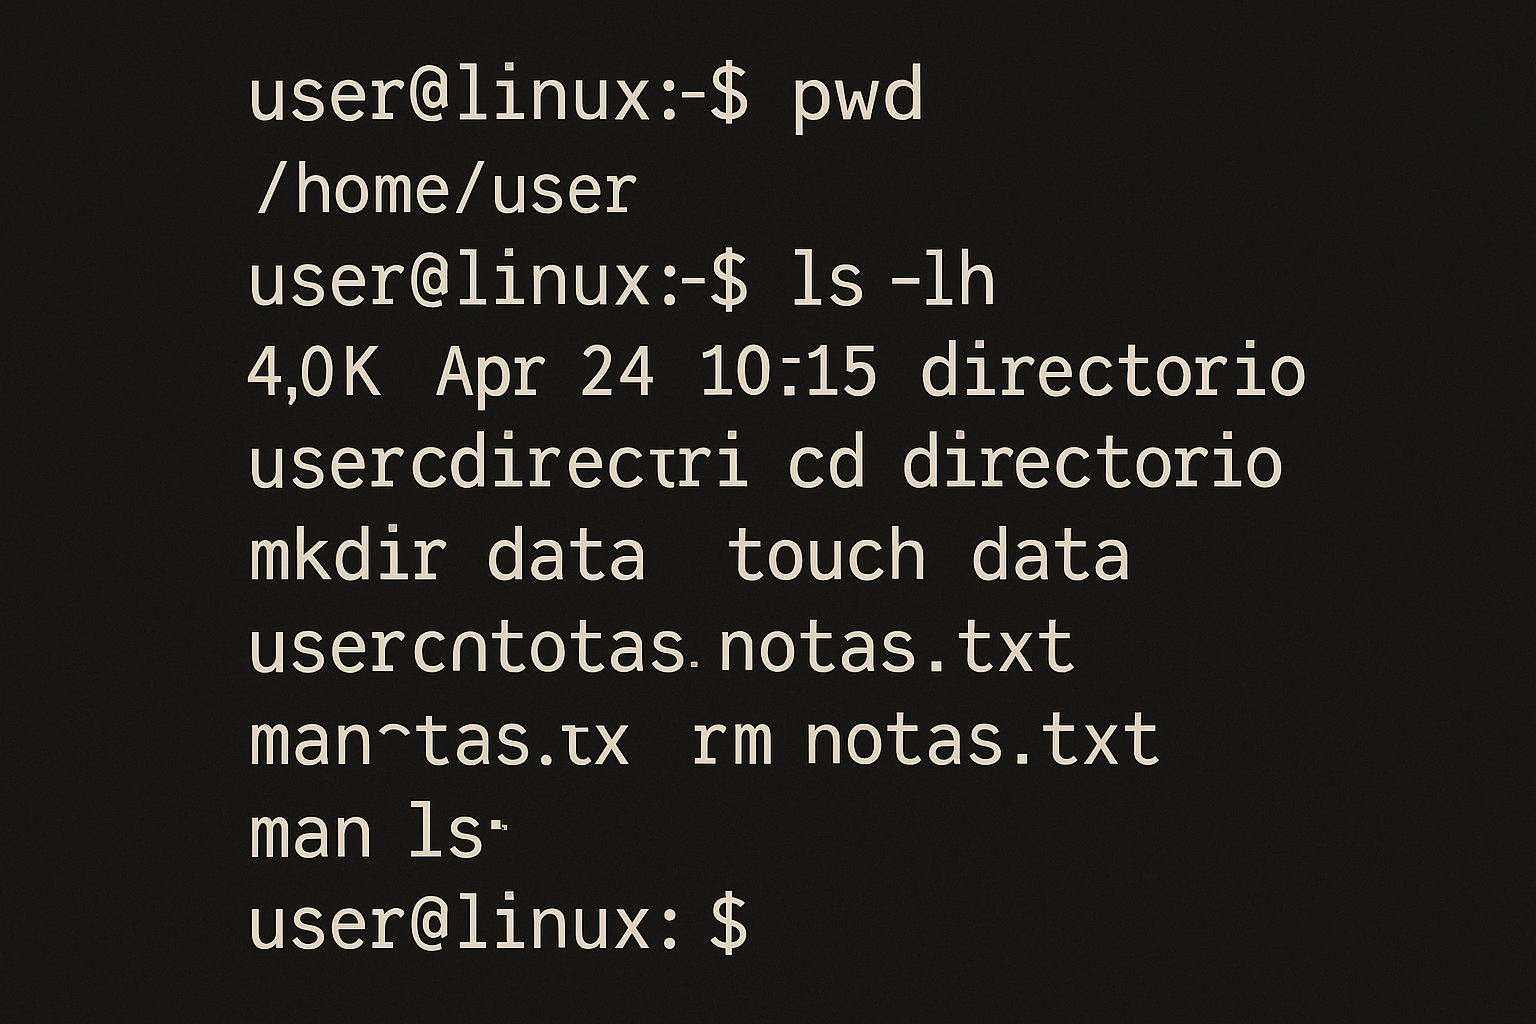
\includegraphics[width=\linewidth]{simple_term.png}
\end{columns}
\end{frame}

%---------------- permisos -------------------------%
\begin{frame}[fragile]{Permisos de archivos}
\begin{minted}{bash}
$ ls -l backup.sh
-rwxr-xr-- 1 pi pi  54 jul  8 12:30 backup.sh
\end{minted}

\begin{itemize}
  \item \texttt{rwx}: propietario
  \item \texttt{r-x}: grupo
  \item \texttt{r--}: otros
\end{itemize}

\begin{warnbox}
  ¡Nunca des permisos 777 salvo que sepas lo que haces!
\end{warnbox}

\begin{minted}{bash}
$ chmod u+x backup.sh        # añadir ejec.
$ sudo chown root:root file  # nuevo dueño
\end{minted}
\end{frame}

%---------------- variables & echo -----------------%
\begin{frame}[fragile]{Variables y \texttt{echo}}
\begin{minted}{bash}
$ NODENAME=$(hostname)
$ echo "Hola, estoy en $NODENAME"
\end{minted}

\begin{minted}{bash}
$ ls -l /etc > listado.txt   # redirige salida
$ cat listado.txt | less     # pipe
\end{minted}
\end{frame}

%---------------- actividad ------------------------%
\begin{frame}{Actividad práctica (30 min)}
\begin{enumerate}
  \item Crear \texttt{~/proyectos/\{scripts,datos,logs\}}
  \item Escribir \texttt{backup.sh} que:
    \begin{itemize}
      \item reciba carpeta (\$1)
      \item comprima con \texttt{tar} \(\to\) \texttt{.tar.gz}
      \item mueva a \texttt{~/backups}
    \end{itemize}
  \item Añadir bit de ejecución y probar.
\end{enumerate}

\small\faLightbulb\; Tip: usa \texttt{\$(date +\%F)} para sellar fecha.
\end{frame}

%---------------- cheatsheet -----------------------%
\begin{frame}[fragile]{Mini cheatsheet}
\begin{columns}[T,onlytextwidth]
\column{0.50\linewidth}
\begin{itemize}
  \item \textbf{Procesos}: \mintinline{bash}{htop}, \mintinline{bash}{ps aux}
  \item \textbf{Disco}: \mintinline{bash}{df -h}, \mintinline{bash}{du -sh *}
  \item \textbf{Buscar}: \mintinline{bash}{grep}, \mintinline{bash}{find}
  \item \textbf{Red}: \mintinline{bash}{ip a}, \mintinline{bash}{ping}
\end{itemize}

\column{0.50\linewidth}
\begin{itemize}
  \item \textbf{Editar}: \mintinline{bash}{nano}, \mintinline{bash}{vim}
  \item \textbf{Actualizar}: \mintinline{bash}{sudo apt update && apt upgrade}
  \item \textbf{Historial}: \mintinline{bash}{history}, \mintinline{bash}{!42}
  \item \textbf{Autocompletar}: ↹ (TAB)
\end{itemize}
\end{columns}
\end{frame}

%---------------- recursos -------------------------%
\begin{frame}{Recursos recomendados}
\begin{itemize}
  \item \emph{The Linux Command Line}, W. Shotts Jr. (ebook gratuito)
  \item \url{https://linuxjourney.com} — interactivo
  \item Documentación oficial de Raspberry Pi OS
\end{itemize}
\end{frame}

%---------------- cierre ---------------------------%
\begin{frame}[plain]
  \centering \Huge ¡Buen trabajo!\\[1ex]
  Siguiente bloque: redes IP y claves SSH
\end{frame}

\end{document}
